\documentclass[11pt]{article}

\usepackage[T1]{fontenc}
\usepackage{lmodern}
\usepackage[a4paper,margin=1.15in]{geometry}
\usepackage{amsmath,amssymb,amsthm}
\usepackage{booktabs}
\usepackage{array}
\usepackage{float}
\usepackage{tikz}
\newcolumntype{P}[1]{>{\raggedright\arraybackslash}p{#1}}
\usepackage{microtype}
\usepackage[hidelinks]{hyperref}

\theoremstyle{definition}
\newtheorem{definition}{Definition}[section]
\theoremstyle{plain}
\newtheorem{proposition}{Proposition}[section]
\theoremstyle{remark}
\newtheorem{remark}{Remark}[section]

\title{Sliding Thermal Carriers for Segmented Accelerators:\\
Heat Transport, Admissibility, and Degraded Operation}
\author{Flyxion\\Independent Researcher}
\date{November 2026}

\begin{document}
\maketitle

\begin{abstract}
\noindent
The heat produced by an accelerator leaves the silicon through a chain of static interfaces, and the temperature at the source is the sum of the drops across them. This essay examines a different arrangement. The accelerator is built as a spine of compute cores, each with a bore, and a conductive carrier is drawn continuously through the bores. The carrier takes up heat by sliding contact, moves it along the spine to a liquid-cooled node, gives it up to the coolant there, and returns cold. The coolant then carries the heat out into a larger substrate, such as a chassis loop or a facility circuit. The essay states the architecture as a definition and derives its steady-state behaviour under explicit assumptions. The temperature of a core depends on the power of every core upstream of it on the carrier, so that thermal admissibility is a global property of the power assignment and cannot be checked core by core. Placing the heaviest loads upstream minimizes the highest steady-state temperature, and a core heats every core downstream of it on the same pass. The number of cores served by one liquid-cooled station bounds the temperature rise accumulated by the carrier, the temperature at which the coolant leaves is bounded above by the temperature of the carrier at the station inlet, and increasing the carrier speed buys less thermal margin as the contact conductance and the coolant take over as the limits. The costs of motion, namely friction heat and wear, and the consequences of a stalled carrier are treated as parts of the specification, together with four measurement protocols that use resistive heaters in place of silicon. A worked example with assumed parameters illustrates each result. No prototype has been built, and the numerical values are assumptions chosen to exercise the model and are not measurements.
\end{abstract}

\section{Introduction}

The power that an accelerator dissipates is bounded in practice by the rate at which heat can be taken away from it. Constant-field scaling of transistors kept the power density of a chip roughly fixed as devices shrank \cite{dennard}, and the end of that regime moved the limit from the switching of the transistors to the removal of heat from the package. Present accelerator racks already use liquid cooling for the whole assembly \cite{nvidia-gb300}, and research on heat removal has long since moved liquid into or next to the silicon \cite{tuckerman,brunschwiler}. The question taken up here is not whether to cool with liquid, since that is settled, but where the moving part of the heat path should be.

In every arrangement mentioned above, the solid between the junction and the coolant is stationary and the fluid moves. The heat must cross a stack of interfaces, namely die, thermal interface material, lid, and cold plate, and the junction temperature is the coolant temperature plus the sum of the drops across the stack. Two consequences follow. A stationary stack has a resistance that the coolant cannot reduce, and a coolant that absorbs the heat of many cores in sequence arrives at the last of them warmer than it left the first. The second consequence is the one that interlayer cooling research identifies as limiting at small channel sizes, where the sensible heat absorbed by the coolant dominates the temperature rise \cite{brunschwiler}.

The arrangement examined in this essay moves a solid. A conductive carrier slides through a bore in each core of a segmented accelerator, and its motion, not the flow of a fluid past the core, is what transports the heat along the spine. A solid of copper stores heat per unit volume at about four fifths of the rate at which water does, so a carrier of modest cross-section moving at a modest speed has an enthalpy capacity comparable to a small coolant flow. At the end of the spine the carrier passes through a liquid-cooled node and is cooled by the coolant, which sweeps the heat into the larger substrate. The carrier is then a closed loop that never leaves the module, and the coolant is the only fluid that does.

The contribution is a specification and an analysis, not a result about a built device. Section~\ref{sec:paths} places the arrangement against existing heat paths. Section~\ref{sec:arch} defines it, and Section~\ref{sec:model} derives its steady-state behaviour. The central finding is a structural one that mirrors a theme of earlier work \cite{flyxion-local}: each core can be acceptable by itself and the assembly can still be inadmissible, because the carrier couples the cores through a shared quantity. Section~\ref{sec:wear} counts the cost of motion. Section~\ref{sec:degraded} treats the failure of the carrier as a case that the module's contract must name. Section~\ref{sec:protocols} gives measurement protocols, and Section~\ref{sec:scope} states what the analysis does not establish.

\section{Heat Paths in Present Accelerators}
\label{sec:paths}

The thermal resistance of a stack is the sum of the resistances of its layers, and the layers that matter most for the present purpose are the interfaces. A review of four decades of work on thermal contact, gap, and joint resistance shows how strongly an interface depends on surface roughness, hardness, pressure, and the fluid between the surfaces \cite{yovanovich}. A static interface is made as good as the clamping force and the filler allow, and then left alone. The interface that this essay introduces is dynamic, and a sliding contact differs from a clamped one in that it must tolerate relative motion for the life of the module. Its conductance is therefore not a property of the materials alone, and Section~\ref{sec:wear} treats it as a quantity that the module must declare and that wear can degrade.

Liquid cooling placed close to the heat source reduces the stack. Water flowing in channels etched into the silicon substrate was demonstrated to remove heat from a chip at very high power density \cite{tuckerman}. For vertically stacked dies, coolant has been routed between the layers, and the performance of such interlayer cooling has been characterized across parallel-plate, microchannel, and pin-fin structures \cite{brunschwiler}. The finding from that work that matters here is that, at small hydraulic diameters, the rise in coolant temperature due to the sensible heat it absorbs limits the cooling performance, and not the convective resistance at the wall. The same accounting appears below with the carrier in place of the coolant: the carrier's temperature rises along the spine by the total power divided by its heat-capacity rate, and every core downstream of another sees that rise.

The comparison with vapour chambers, heat pipes, and oscillating heat pipes is taken up in Section~\ref{sec:related}, after the model has been stated, because the comparison depends on which quantities the model makes explicit.

\section{A Segmented Accelerator with Sliding Carriers}
\label{sec:arch}

The accelerator is an ordered sequence of $n$ cores along a spine. Each core is a compute element with a bore, a channel that passes through it along the axis of the spine. A carrier is a conductive rod, band, or chain that passes through the bore of every core in order. It is driven so that it moves continuously in one direction along the spine, and it closes on itself by a return path outside the cores, so that no carrier material leaves the module.

\begin{figure}[t]
\centering
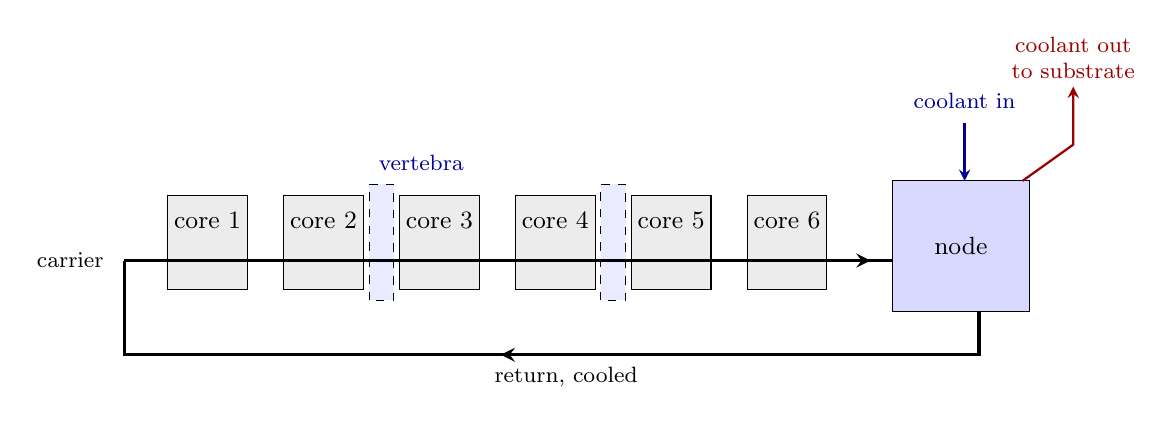
\begin{tikzpicture}[x=1cm,y=1cm,>=stealth,font=\small,scale=0.92]
  % cores
  \foreach \i in {1,2,3,4,5,6} {
    \draw[fill=gray!15] ({(\i-1)*1.6},0) rectangle ({(\i-1)*1.6+1.1},1.3);
    \node at ({(\i-1)*1.6+0.55},0.95) {core $\i$};
  }
  % vertebra markers between cores
  \foreach \x in {2.78,5.98} {
    \draw[fill=blue!8,dashed] (\x,-0.15) rectangle (\x+0.34,1.45);
  }
  \node[blue!60!black,font=\footnotesize] at (3.5,1.75) {vertebra};
  % carrier path, drawn over the cores
  \draw[very thick] (-0.6,0.4) -- (9.7,0.4);
  \draw[very thick,->] (8.4,0.4) -- (9.7,0.4);
  \node[font=\footnotesize,anchor=east] at (-0.75,0.4) {carrier};
  % node
  \draw[fill=blue!15] (10.0,-0.3) rectangle (11.9,1.5);
  \node at (10.95,0.6) {node};
  \draw[very thick] (9.7,0.4) -- (10.0,0.4);
  % return path
  \draw[very thick] (11.2,-0.3) -- (11.2,-0.9) -- (-0.6,-0.9) -- (-0.6,0.4);
  \draw[very thick,->] (5,-0.9) -- (4.6,-0.9);
  \node[font=\footnotesize] at (5.5,-1.2) {return, cooled};
  % coolant
  \draw[->,thick,blue!60!black] (11.0,2.3) -- (11.0,1.5);
  \node[blue!60!black,font=\footnotesize] at (11.0,2.6) {coolant in};
  \draw[->,thick,red!60!black] (11.8,1.5) -- (12.5,2.0) -- (12.5,2.8);
  \node[red!60!black,font=\footnotesize,align=center] at (12.5,3.2) {coolant out\\to substrate};
\end{tikzpicture}
\caption{Schematic of the spine for $n=6$. The carrier enters the first bore at temperature $\theta_0$, takes up heat in each core in turn, reaches the node at temperature $\theta_n$, and returns cooled. Dashed regions mark vertebrae, the coolant-bearing elements that may hold additional stations between cores.}
\label{fig:spine}
\end{figure}

The terms of the design are fixed by the following definition. The name \emph{vertebra} is used for the coolant-bearing element of the spine, since a series of such elements along the axis, with the carrier passing through all of them, is what gives the structure its articulated form. The \emph{node} is the vertebra at which the carrier's heat is finally delivered to the coolant of the module, and the \emph{substrate} is the larger body that receives the coolant afterwards.

\begin{definition}[Segmented accelerator with sliding carriers]\label{def:seg}
A segmented accelerator with sliding carriers consists of the following.
\emph{Cores} $1,\dots,n$ in carrier order, with powers $P_1,\dots,P_n\ge 0$. Each core $i$ has a junction resistance $R_j$ between the junction and the bore wall, so that the junction is at the wall temperature plus $R_jP_i$.
\emph{Carriers}, which move at speed $v$ and together have heat-capacity rate $C=\rho c A v\, m$, where $\rho c$ is the volumetric heat capacity of the carrier material, $A$ the cross-section of one carrier, and $m$ the number of carriers in parallel.
\emph{Bore contacts}, each with conductance $G$ between the carriers and the bore wall of a core, and the dimensionless number $\varepsilon=1-e^{-G/C}$ that results.
\emph{Stations}, which are vertebrae in which the carrier exchanges heat with a coolant stream of capacity rate $C_w$ and inlet temperature $T_w$, with effectiveness $\varepsilon_N$.
A temperature limit $T_{\max}$ applies to every junction.
\end{definition}

\begin{remark}[Reciprocating variant]
A set of short sliders that shuttle between a hot position and a cold position transports heat with the same mean heat balance. A slider of mass $M_s$ and specific heat $c$ that completes $f$ cycles per unit time, absorbing heat at its hot position and releasing it at its cold position, carries $M_s c\,\Delta T f$ per unit time, which is the form $Q=C\Delta T$ with $C=M_s c f$. Only this mean balance is claimed. Extending the profile of Proposition~\ref{prop:profile} and the ordering of Proposition~\ref{prop:order} to a shuttle would require assumptions about when it contacts each core, how completely it cools between strokes, and the temperature ripple within a cycle. The shuttle is therefore a second architecture, whose equivalence to the continuous loop is a matter to be tested, and the analysis below is for the continuous loop.
\end{remark}

\begin{remark}[Electrical isolation]
A metal carrier that touches the bore of an active core must be electrically isolated from it. The isolating layer adds a series resistance to the contact, and the conductance $G$ of Definition~\ref{def:seg} is the conductance of the whole interface, isolation included. A carrier made of a dielectric of high thermal conductivity avoids the layer and has a lower heat capacity per unit volume. The analysis below does not depend on the choice, and the choice enters through $\rho c$ and $G$.
\end{remark}

\begin{remark}[Substrate]
The substrate is whatever receives the coolant after the node: a chassis plate network, a rack manifold, or a building circuit. The module's contract concerns its coolant inlet and outlet. The analysis treats the substrate as supplying coolant at temperature $T_w$ and capacity rate $C_w$ and does not model it further.
\end{remark}

\section{Steady-State Heat Transport}
\label{sec:model}

The model rests on four assumptions, which are stated here because the propositions are conditional on them.

The first assumption, A1, is that the module is at steady state and every core dissipates its power $P_i$ entirely into the carrier, so that other heat paths from the cores, such as conduction into the spine structure, are neglected. The second, A2, is that each bore wall is isothermal and exchanges with the carrier stream according to the effectiveness relation for a stream passing an isothermal surface \cite{kayslondon}, so that the heat taken up in core $i$ is $\varepsilon C(T_i-\theta_{i-1})$, where $T_i$ is the wall temperature and $\theta_{i-1}$ the carrier temperature on entry to the bore. The third, A3, is that axial conduction along the carrier is negligible against its advection. For a copper carrier of $4\times 9\ \mathrm{mm}^2$ total cross-section over a spine length of $0.1$ m, the conductance $kAm/L$ is about $0.14$ W/K, against $C\approx 62$ W/K for the example of Section~\ref{sec:example}, a ratio near $0.2$ percent. The fourth, A4, is that the carrier is returned to a fixed entry temperature $\theta_0$ by the station that precedes the first core.

\begin{proposition}[Carrier profile]\label{prop:profile}
Under A1 to A4, the carrier temperature on leaving core $i$ is $\theta_i=\theta_{i-1}+P_i/C$, and the junction temperature of core $i$ is
\[
T^{\mathrm{J}}_i \;=\; \theta_0 \;+\; \frac1C\sum_{j<i}P_j \;+\; P_i\,a,
\qquad a=\frac{1}{\varepsilon C}+R_j .
\]
\end{proposition}
\begin{proof}
At steady state the heat taken up by the carrier in core $i$ equals $P_i$, so the energy balance of the carrier through the bore is $C(\theta_i-\theta_{i-1})=P_i$. By A2 the same heat is $\varepsilon C(T_i-\theta_{i-1})$, which gives $T_i=\theta_{i-1}+P_i/(\varepsilon C)$ for the wall. Summing the balances from the first core gives $\theta_{i-1}=\theta_0+\frac1C\sum_{j<i}P_j$, and adding the junction offset $R_jP_i$ gives the stated expression.
\end{proof}

The expression has two terms that depend on the powers. The term $P_i a$ depends on the core alone, and the term $\frac1C\sum_{j<i}P_j$ depends on every core upstream. The second term is what makes the assembly more than the sum of its cores.

\begin{definition}[Local and global admissibility]
Core $i$ is \emph{locally admissible} at power $P_i$ if $\theta_0+P_ia\le T_{\max}$, which is the condition for the core to meet the limit when it alone dissipates. A power assignment is \emph{globally admissible} if $T^{\mathrm J}_i\le T_{\max}$ for every $i$.
\end{definition}

\begin{proposition}[Global admissibility is strictly stronger]\label{prop:global}
If $P_j>0$ for some $j<i$, then $T^{\mathrm J}_i$ exceeds the local value $\theta_0+P_ia$ by $\frac1C\sum_{j<i}P_j>0$, so global admissibility of core $i$ implies local admissibility of core $i$ and the converse fails. Moreover, the node couples the cores further: the entry temperature $\theta_0$ is itself a nondecreasing function of the total power $Q=\sum_i P_i$.
\end{proposition}
\begin{proof}
The first statement is read directly from Proposition~\ref{prop:profile}. For the second, the carrier delivers $Q$ to the coolant at the node, so $Q=\varepsilon_N C_{\min}(\theta_n-T_w)$ with $C_{\min}=\min(C,C_w)$, and $\theta_n=\theta_0+Q/C$. Eliminating $\theta_n$ gives $\theta_0=T_w+Q\left(\frac{1}{\varepsilon_N C_{\min}}-\frac1C\right)$. Because $C_{\min}\le C$ and $\varepsilon_N\le1$, the bracket $\frac{1}{\varepsilon_N C_{\min}}-\frac1C$ is nonnegative, so $\theta_0$ is nondecreasing in $Q$.
\end{proof}

The proposition has the form of the earlier observation that local transitions can each be admissible while the global configuration is not \cite{flyxion-local}. Here the shared quantity is the carrier's heat content, and the boundary through which the cores exchange is the carrier itself.

\begin{proposition}[Ordering]\label{prop:order}
Among all orderings of a fixed multiset of core powers along the carrier, the ordering with powers in nonincreasing order minimizes the steady-state peak $\max_i T^{\mathrm J}_i$.
\end{proposition}
\begin{proof}
The total power $Q$ and hence $\theta_0$ are the same for every ordering, so the comparison concerns the profile of Proposition~\ref{prop:profile} with $b=1/C$ and $a\ge b$, where $a-b=\frac{1}{\varepsilon C}-\frac1C+R_j\ge0$ because $\varepsilon\le1$. Consider two adjacent cores holding $P<P'$ in that order, and let $X=\theta_0+\frac1C S$ with $S$ the power upstream of the pair. Before an exchange the two junctions are at $X+aP$ and $X+bP+aP'$, and the larger is $X+bP+aP'$. After exchanging, they are at $X+aP'$ and $X+bP'+aP$. The first is at most $X+bP+aP'$, and the second is at most $X+bP+aP'$ because $(bP+aP')-(bP'+aP)=(a-b)(P'-P)\ge0$. The cores upstream of the pair see the same upstream power, and the cores downstream see the same total upstream power, so no other junction changes. Any ordering in which a smaller power precedes a larger one can be improved or left unchanged by such an exchange, and repeated exchanges reach the nonincreasing order without raising the maximum.
\end{proof}

The proposition concerns the peak steady-state temperature and nothing else. The dependence it describes is directional: a core heats every core downstream of it on the same pass, and the finite station returns part of the total load to the inlet temperature of the next pass. It does not say which ordering gives the best response to a stall, which depends on the thermal mass, power, and margin of each core together, as Section~\ref{sec:degraded} shows.

\begin{proposition}[Stations bound the accumulated rise]\label{prop:stations}
Suppose a station returns the carrier to $\theta_0$ after every $k$ cores, with the same $\theta_0$ at each. Then for every core the junction temperature satisfies
\[
T^{\mathrm J}_i \;\le\; \theta_0+\frac{(k-1)\,P_{\max}}{C}+P_{\max}\,a,
\]
a bound that does not depend on $n$, where $P_{\max}=\max_iP_i$.
\end{proposition}
\begin{proof}
Within a group of $k$ cores the upstream sum in Proposition~\ref{prop:profile} contains at most $k-1$ terms, each at most $P_{\max}$.
\end{proof}

The proposition is the sense in which the vertebrae matter. A single node at the end of a spine of $n$ cores accumulates a rise of $(n-1)P/C$ for uniform power, and stations placed between cores cut the rise to $(k-1)P/C$ at the price of one liquid-cooled element for every $k$ cores. The coolant is the other side of the same trade, and the next proposition states it.

\begin{proposition}[Heat-grade ceiling]\label{prop:grade}
The temperature at which the coolant leaves the node cannot exceed the carrier temperature at the node inlet, and that temperature is itself bounded by the junction limit:
\[
T_{w,\mathrm{out}}\;\le\;\theta_n\;\le\;T_{\max}-R_jP_n-P_n\!\left(\frac{1}{\varepsilon C}-\frac1C\right).
\]
\end{proposition}
\begin{proof}
A passive exchanger cannot heat the coolant above the inlet temperature of the hotter stream, which is the first inequality. For the second, $\theta_n=\theta_{n-1}+P_n/C$ while the wall of the last core is at $\theta_{n-1}+P_n/(\varepsilon C)$ and its junction at that value plus $R_jP_n$. The junction is at most $T_{\max}$, and rearranging gives the bound.
\end{proof}

The proposition says that the heat of the module can be delivered at a high temperature only if the cores run close to their limit. When the heat is wanted at a particular temperature, for example for a hydronic heating circuit, the temperature that the module can offer is limited by the same $T_{\max}$ that limits the cores, and the number of cores per station, $k$, determines how much of that limit the carrier uses.

\subsection{A worked example}
\label{sec:example}

Table~\ref{tab:params} gives the parameters of the example. The values are assumptions chosen to exercise the model. The contact coefficient and the junction resistance in particular are placeholders for quantities that Section~\ref{sec:protocols} proposes to measure.

\begin{table}[t]
\centering
\small
\begin{tabular}{@{}P{5.7cm}P{6.9cm}@{}}
\toprule
Quantity & Value \\
\midrule
Cores, power & $n=8$, $P_i=250$ W (total $Q=2000$ W) \\
Carrier & copper, $3\times3$ mm, $m=4$ in parallel, $v=0.5$ m/s \\
Volumetric heat capacity, heat-capacity rate & $\rho c=3.45$ MJ/(m$^3$K), $C=62.1$ W/K \\
Bore contact & $2.4\times10^{-4}$ m$^2$ per carrier per core, $5\times10^{4}$ W/(m$^2$K), so $G=48.0$ W/K \\
Effectiveness & $G/C=0.773$, $\varepsilon=0.538$ \\
Junction resistance, limit & $R_j=0.06$ K/W, $T_{\max}=95\ ^\circ$C \\
Coolant & water, 1.5 L/min, $C_w=104.5$ W/K, inlet $T_w=35\ ^\circ$C \\
Node effectiveness & $\varepsilon_N=0.9$ \\
Core thermal mass (Section~\ref{sec:degraded}) & $K_c=150$ J/K \\
\midrule
Derived: carrier rise, entry, node inlet & $Q/C=32.2$ K, $\theta_0=38.6\ ^\circ$C, $\theta_n=70.8\ ^\circ$C \\
Derived: coolant outlet & $T_w+Q/C_w=54.1\ ^\circ$C \\
\bottomrule
\end{tabular}
\caption{Parameters of the worked example. All values are assumptions.}
\label{tab:params}
\end{table}

With uniform power the junction temperatures of Proposition~\ref{prop:profile} rise by $P/C=4.03$ K from core to core, from $61.1\ ^\circ$C at the first core to $89.2\ ^\circ$C at the eighth, below the limit of $95\ ^\circ$C. The coolant leaves at $54.1\ ^\circ$C, which is below the ceiling of Proposition~\ref{prop:grade}, equal to $76.5\ ^\circ$C for $P_n=250$ W.

The gap between local and global admissibility is large here. Taken alone, with the carrier entering at the example's $\theta_0=38.6\ ^\circ$C, a core meets the limit up to about $627$ W. This is a local screening limit with the inlet held fixed. A single powered core on the same closed loop changes the station load and so its own inlet temperature, and with the parameters of Table~\ref{tab:params} the isolated-core limit is about $654$ W. With all eight cores dissipating, the largest uniform power that keeps every junction below the limit is about $276$ W, because the last core carries the accumulated rise and the node raises $\theta_0$ with the total. At $300$ W per core every core is locally admissible and the eighth reaches $100.1\ ^\circ$C.

Ordering matters at fixed total power. Table~\ref{tab:order} gives the same $2000$ W distributed unevenly over the eight cores. With the heaviest cores first, the highest junction is at $81.8\ ^\circ$C. With the reverse order, the same powers drive the last core to $104.0\ ^\circ$C and the assembly is inadmissible, though the largest single power is $450$ W, well below the local limit.

\begin{table}[t]
\centering
\small
\begin{tabular}{@{}lcccccccc@{}}
\toprule
Core & 1 & 2 & 3 & 4 & 5 & 6 & 7 & 8 \\
\midrule
Power, heavy first (W) & 450 & 400 & 300 & 250 & 200 & 150 & 150 & 100 \\
Junction ($^\circ$C) & 79.0 & 81.8 & 79.2 & 79.6 & 79.1 & 77.8 & 80.2 & 78.2 \\
\midrule
Power, heavy last (W) & 100 & 150 & 150 & 200 & 250 & 300 & 400 & 450 \\
Junction ($^\circ$C) & 47.6 & 53.7 & 56.1 & 63.0 & 70.7 & 79.2 & 93.1 & 104.0 \\
\bottomrule
\end{tabular}
\caption{The same eight powers in opposite orders. The maximum is $81.8\ ^\circ$C with the heaviest cores upstream and $104.0\ ^\circ$C with them downstream. The limit is $95\ ^\circ$C.}
\label{tab:order}
\end{table}

Stations change the picture, as Table~\ref{tab:stations} shows for uniform $250$ W with the return temperature imposed at $38.6\ ^\circ$C. A station after every second core reduces the highest junction from $89.2\ ^\circ$C to $65.1\ ^\circ$C, and the carrier reaches the station inlet at only $46.7\ ^\circ$C. By Proposition~\ref{prop:grade} the coolant leaving such a station cannot be warmer than that. The cooler cores are paid for in lower heat grade, which is the trade named after the proposition.

\begin{table}[t]
\centering
\small
\begin{tabular}{@{}rcc@{}}
\toprule
Cores per station $k$ & Highest junction ($^\circ$C) & Carrier at station inlet ($^\circ$C) \\
\midrule
1 & 61.1 & 42.6 \\
2 & 65.1 & 46.7 \\
4 & 73.1 & 54.7 \\
8 & 89.2 & 70.8 \\
\bottomrule
\end{tabular}
\caption{Effect of station spacing for uniform $250$ W, with the carrier returned to $38.6\ ^\circ$C at each station. That return temperature is imposed. A comparison at fixed coolant inlet, flow, and station effectiveness would solve for the return temperature of each configuration. The right column bounds the temperature of the coolant leaving a station.}
\label{tab:stations}
\end{table}

\subsection{Carrier speed}
\label{sec:speed}

At fixed contact conductance $G$, the carrier speed enters the model through $C\propto v$ alone, and the two terms of Proposition~\ref{prop:profile} respond differently to it.

\begin{proposition}[Diminishing return of speed]\label{prop:speed}
Fix $G$, $R_j$, the core powers, and the coolant. As $C\to\infty$, the upstream term $\frac1C\sum_{j<i}P_j$ tends to zero and $\frac{1}{\varepsilon C}=\frac{1}{C(1-e^{-G/C})}$ tends to $\frac1G$, so the local wall-to-carrier drop tends to $P_i/G$ and does not vanish. For $C>C_w$ the minimum capacity rate in the node is the coolant's, and $\theta_0$ tends to $T_w+Q/(\varepsilon_N C_w)$. The friction power $\mu N v$ per contact grows linearly in $v$ at fixed $N$ and $\mu$.
\end{proposition}
\begin{proof}
Both limits follow from $C(1-e^{-G/C})\to G$ as $C\to\infty$. The node relation of Proposition~\ref{prop:global} with $C_{\min}=C_w$ gives the limit of $\theta_0$, since $Q/C\to0$.
\end{proof}

Table~\ref{tab:speed} gives the last core of the example over a range of speeds. Friction heat is listed and is not included in the junction temperatures. From $0.25$ to $1$ m/s the highest junction falls from $123.8\ ^\circ$C to $75.5\ ^\circ$C. Beyond $1$ m/s it stops falling, because the upstream rise has become small and the wall drop and coolant terms dominate, while the friction power doubles with each doubling of speed, from $64$ W at $1$ m/s to $256$ W at $4$ m/s. In the example the speed at which additional motion stops buying thermal margin is near $1$ m/s, and the sweep of Run H1 below measures where it lies in a real module.

\begin{table}[t]
\centering
\small
\begin{tabular}{@{}rcccc@{}}
\toprule
$v$ (m/s) & $C$ (W/K) & $\varepsilon$ & Highest junction ($^\circ$C) & Friction power (W) \\
\midrule
0.25 & 31.0 & 0.787 & 123.8 & 16 \\
0.5 & 62.1 & 0.538 & 89.2 & 32 \\
1 & 124.2 & 0.321 & 75.5 & 64 \\
2 & 248.4 & 0.176 & 76.0 & 128 \\
4 & 496.7 & 0.092 & 76.2 & 256 \\
\bottomrule
\end{tabular}
\caption{Carrier speed for the example of Table~\ref{tab:params}, uniform $250$ W. The limiting value as $v\to\infty$ is $76.5\ ^\circ$C. Friction heat is not included in the junction temperatures and would add to the node load.}
\label{tab:speed}
\end{table}

\section{Friction, Wear, and the Cost of Motion}
\label{sec:wear}

The carrier moves, so the sliding contacts dissipate power and lose material. Both effects can be bounded with simple relations, and both depend on parameters that this essay assumes and does not measure.

\paragraph{Friction heat.} A contact carrying normal force $N$ at sliding speed $v$ with friction coefficient $\mu$ dissipates $\mu N v$. For a lubricated or liquid-metal-wetted interface with $\mu=0.1$, $N=20$ N, and $v=0.5$ m/s, each contact dissipates $1.0$ W. The example has $8\times 4=32$ contacts, so the friction power is $32$ W, which is $1.6$ percent of the $2000$ W of the cores. It enters the node load and the carrier rise, and it is the power that the carrier drive must supply. A design in which the friction power approaches a few percent of the load would be spending a significant part of its cooling capacity on its own motion.

\paragraph{Wear.} The classical relation attributes a wear volume $V=KNs/H$ to a contact of hardness $H$ under load $N$ over a sliding distance $s$, with a dimensionless wear coefficient $K$ \cite{archard}. At $0.5$ m/s the carrier slides $1.58\times10^{7}$ m in a year. With $N=20$ N, $H=1$ GPa, and the contact area $2.4\times10^{-4}$ m$^2$ of the example, the depth removed per contact in a year is $1.3\ \mu$m for $K=10^{-9}$, $131\ \mu$m for $K=10^{-7}$, and $1.3$ mm for $K=10^{-6}$. These span three orders of magnitude, from negligible to destructive, and the span is the point: the wear coefficient decides whether the architecture is practical, and its value for the chosen pair of materials and film is an experimental question that no relation in this essay settles.

\paragraph{Contact conductance over life.} Wear changes the surface, and debris changes the interface. The conductance $G$ of Definition~\ref{def:seg} therefore drifts, and its drift enters the model through $\varepsilon=1-e^{-G/C}$. Lower $G$ raises $a$ and all junction temperatures by Proposition~\ref{prop:profile}, with the largest effect on the cores that already run closest to the limit. The module's contract should state a floor on $G$ and the rated life over which it holds, and the protocol of Section~\ref{sec:protocols} that tests it records the drift of $G$ with sliding distance.

\section{Degraded Operation and the Thermal Contract}
\label{sec:degraded}

A carrier can stop. The drive can fail, a contact can seize, or debris can jam the return path. In that case A1 no longer describes the module, because the cores lose their path to the node except through whatever residual conduction the structure provides. The specification must say what the module promises when this happens, in the same way that a module of a cloud service must say what it does when a link fails \cite{flyxion-gpu}.

Let $T^{\mathrm J}_i$ be the junction temperature of core $i$ at the moment of the stall, let $K_{c,i}$ be an effective thermal mass for core $i$, and suppose the core continues at power $P_i$. In a lumped model in which the core is a single temperature, loses no heat, and receives no heat from its neighbours, its temperature rises at $P_i/K_{c,i}$ and reaches the limit after
\[
t_i \;=\; \frac{K_{c,i}\,(T_{\max}-T^{\mathrm J}_i)}{P_i}.
\]
The formula is exact for that model. Whether it is a safe estimate for a real junction depends on two things that the model assumes and does not show: that $K_{c,i}$ represents the thermal mass actually coupled to the junction over the response interval, which for a small junction heated at high flux can be much less than the mass of the whole core, and that heat flowing in from neighbouring components or from the stalled carrier cannot raise the temperature faster than the lumped rate. A heater block, which has a larger and more uniform mass than a junction, can show a slower transient than the device it stands for. For these reasons the next proposition is stated as a result of the lumped model.

\begin{proposition}[Safe response time, lumped model]\label{prop:stall}
In the lumped model, suppose the module detects a stall and reduces every core to a power that its residual path can sustain within a time $t_d$ after the stall. Then no core exceeds $T_{\max}$ provided $t_d\le\min_i t_i$, where each $t_i$ is computed from a positive margin $T_{\max}-T^{\mathrm J}_i>0$.
\end{proposition}
\begin{proof}
Until time $t_d$ core $i$ heats at $P_i/K_{c,i}$, so its temperature at $t_d$ is $T^{\mathrm J}_i+P_it_d/K_{c,i}\le T_{\max}$ when $t_d\le t_i$. After the reduction the power is sustainable by assumption.
\end{proof}

The proposition needs a positive margin. A core assigned exactly to $T_{\max}$ has $t_i=0$, and no response is fast enough, so a module that is operated at its limit has no stall response to declare and must not be operated there when a stall is possible.

In the worked example, with $K_{c,i}=150$ J/K assumed for every core, the margins of Proposition~\ref{prop:profile} give $t_1=20.3$ s for the first core and $t_8=3.5$ s for the last. The response time that this module would have to meet is $3.5$ s, set by the core with the least margin per unit of $P_i/K_{c,i}$. Which core that is depends on all three quantities. The ordering of Proposition~\ref{prop:order} minimizes the steady-state peak and says nothing about $\min_i t_i$. An assignment that maximizes the stall response time would be the solution of a separate problem, the maximization of $\min_i K_{c,i}(T_{\max}-T^{\mathrm J}_i)/P_i$ over assignments, and that problem is not solved here. A speed sensor on the drive detects a stall within milliseconds at $0.5$ m/s, which is far inside the budget, and the budget that matters is the one for actuation, since reducing power across all cores through the accelerator's own power management must also finish within it.

\begin{table}[t]
\centering
\small
\begin{tabular}{@{}P{2.6cm}P{3.4cm}P{3.4cm}P{3.4cm}@{}}
\toprule
Mode & Observable & Effect on the model & Required response \\
\midrule
Carrier stall or seizure & Speed sensor reads zero, drive current rises & $C\to0$, A1 fails & Reduce power within $\min_i t_i$, report fault \\
Contact degradation & Rise of wall temperature at fixed power & $G$ falls, $\varepsilon$ falls & Derate by Proposition~\ref{prop:profile}, report drift \\
Coolant loss or reduced flow & Node inlet temperature rises & $C_w$ falls, $\theta_0$ rises & Derate by Proposition~\ref{prop:global}, report \\
Debris or leak in the return path & Rise of drive power, particle count & $\mu$ rises, $G$ may change & Stop in a safe state, report \\
\bottomrule
\end{tabular}
\caption{Failure modes of the carrier loop, their observables, their effect on the model, and the response the contract requires.}
\label{tab:modes}
\end{table}

Table~\ref{tab:modes} lists the failure modes together with what each does to the model and what the module must do. For a module in a cloud service the response includes a report to the scheduler. A stall is a fault of the module, and an application running on it is subject to the same recovery contract as for any other fault of a module: a typed outcome, either a commit before the module withdraws or a suspension that can resume from the last committed checkpoint \cite{flyxion-gpu}. The thermal contract adds the quantities that must be declared for the response to be checkable, namely the response time $t_d$ and the sustainable power after a stall.

\section{Relation to Other Heat Paths}
\label{sec:related}

A cold plate on a static interface has a junction temperature that is the coolant temperature plus the drops across the stack. It has no carrier rise, since the coolant flows past each cold plate in parallel, and its limit is the resistance of the stack. A vapour chamber or heat pipe spreads heat by evaporation and condensation within a sealed envelope, and moves it to a condenser with a small temperature difference. It has no moving solid, and its transport capacity is limited by the working fluid and wick. An oscillating or pulsating heat pipe moves heat by the motion of vapour plugs and liquid slugs in a capillary tube, and its behaviour is hard to predict in general. Microchannel and interlayer cooling bring the liquid to the silicon \cite{tuckerman,brunschwiler}. The sliding carrier replaces none of these. Its distinctive feature is that heat is moved along the spine by the motion of a solid that returns, so that the interface to each core is a dynamic one, and its distinctive costs are the contact, friction, and wear terms of Section~\ref{sec:wear}.

The comparison that would decide between these paths is a comparison of measured junction temperature at equal power, equal coolant, and equal lifetime. The model in this essay supplies the prediction for the sliding carrier, and the protocols below supply the measurement. No claim is made here that the sliding carrier performs better than any of the alternatives.

\section{Evaluation Protocols}
\label{sec:protocols}

The protocols use resistive heaters in place of silicon, so that the power of each core is set and measured directly. Each is stated in the form \emph{initial checkpoint}, \emph{varied}, \emph{injected}, \emph{recorded}, \emph{passes when}.

\paragraph{Run H1, carrier profile.} \emph{Initial checkpoint.} Eight heater cores on a spine with the carrier at its nominal speed and the coolant at its nominal inlet temperature and flow. \emph{Varied.} The carrier speed over at least five values, and the power per core over at least three values. \emph{Injected.} None. \emph{Recorded.} The wall temperature of each core, the carrier temperature at each bore inlet, the node inlet and outlet temperatures, the drive power, and the friction power at each speed. The bore-wall and carrier temperatures identify $G$ under the model, and $R_j$ is identified only if a temperature is also recorded on the heater side of the junction-equivalent resistance, or if that resistance is calibrated independently before the run. \emph{Passes when.} The fitted value of $G$, taken from the runs at one speed, predicts the wall temperatures at the other speeds within a tolerance stated before the run, the carrier temperature rise from core to core is $P/C$ within the stated tolerance, and the sweep reports the speed beyond which the highest junction-equivalent temperature falls by less than a stated amount per added watt of friction power, which is the measured counterpart of Proposition~\ref{prop:speed}.

\paragraph{Run H2, ordering.} \emph{Initial checkpoint.} As H1 at the nominal speed. \emph{Varied.} The assignment of a fixed set of heater powers to positions, between the order of nonincreasing power and its reverse, and at least one intermediate order. \emph{Injected.} None. \emph{Recorded.} The highest junction-equivalent temperature for each order. \emph{Passes when.} The nonincreasing order produces the lowest recorded maximum, as Proposition~\ref{prop:order} requires, and the recorded maxima agree with the predictions of Proposition~\ref{prop:profile} within the tolerance.

\paragraph{Run H3, stall.} \emph{Initial checkpoint.} As H1, with the heaters at an assignment that leaves a stated positive margin $\delta>0$ below $T_{\max}$ at every core. \emph{Varied.} The time of the stall within the run, the heater power at the time of the stall, and the margin $\delta$ over at least three values. \emph{Injected.} The carrier is stopped at a recorded time. In a second condition the drive is released so that it resumes. \emph{Recorded.} A junction-equivalent temperature for each core, taken on the heater side of the junction resistance and sampled fast enough to resolve the response interval, together with the detection time, the time at which power is reduced, and the peak temperature of each core. The effective thermal mass $K_{c,i}$ is fitted from the recorded transient over the response interval and is compared with the value the contract declares. \emph{Passes when.} The peak temperature of every core stays below $T_{\max}$, the fitted $K_{c,i}$ is not larger than the declared value, so that the rig is not slower than the device it represents, the recorded response time is at most $\min_it_i$ computed from the fitted values and the measured margins, and the resumed carrier restores the profile of H1 within the tolerance.

\paragraph{Run H4, contact life.} \emph{Initial checkpoint.} As H1, with a new carrier and bores. \emph{Varied.} The sliding distance, in stated increments up to the rated life. \emph{Injected.} A controlled quantity of debris in the return path in one condition. \emph{Recorded.} The conductance $G$ fitted at each increment, the friction power, the wear depth measured on the carrier and the bore at the end, and the particle count in the loop. \emph{Passes when.} $G$ remains above the declared floor and the friction power below the declared ceiling throughout, and the measured wear depth is consistent with the wear coefficient that the declared life assumes.

\section{What the Model Does Not Establish}
\label{sec:scope}

The essay specifies an architecture and derives its behaviour from assumptions. It does not report a measurement. The values of the contact conductance, the junction resistance, the friction coefficient, and the wear coefficient are assumed, and Section~\ref{sec:wear} shows that the last of them alone spans the range from irrelevant to disqualifying. The model is steady-state, and the transient behaviour of the carrier as it enters a bore that is hot or cold, which matters for fast changes of load, is not modelled beyond the lumped estimate of Proposition~\ref{prop:stall}, which holds for a single-temperature core with no heat inflow from its neighbours and is to be checked against a measured junction-equivalent transient. The analysis treats each core as a single lumped element with an isothermal bore, and the temperature variation inside a real core, including hot spots, enters only through the single resistance $R_j$.

The mechanical questions are outside the analysis. A driven loop of conductor inside a sealed accelerator must be sealed against the coolant, must not shed particles near the electronics, and must tolerate thermal expansion across the spine, and none of these is addressed. The electrical isolation of the carrier from the cores is a requirement stated in Section~\ref{sec:arch} and not a design. A comparison of the architecture with the cold plate, the vapour chamber, or interlayer cooling on measured performance is deferred to experiments that the protocols describe, and the essay makes no claim about their outcome. Finally, the essay concerns the heat path of a module, and what a cloud service should promise about it is a matter for the contract that surrounds the module \cite{flyxion-gpu}.

\begingroup
\small
\setlength{\itemsep}{0pt}
\begin{thebibliography}{99}

\bibitem{archard}
Archard, J. F.
\newblock Contact and Rubbing of Flat Surfaces.
\newblock \emph{Journal of Applied Physics}, 24(8):981--988, 1953.
\newblock doi:10.1063/1.1721448.

\bibitem{brunschwiler}
Brunschwiler, T., Michel, B., Rothuizen, H., Kloter, U., Wunderle, B., Oppermann, H., and Reichl, H.
\newblock Interlayer Cooling Potential in Vertically Integrated Packages.
\newblock \emph{Microsystem Technologies}, 15:57--74, 2009.
\newblock doi:10.1007/s00542-008-0690-4.

\bibitem{dennard}
Dennard, R. H., Gaensslen, F. H., Yu, H.-N., Rideout, V. L., Bassous, E., and LeBlanc, A. R.
\newblock Design of Ion-Implanted MOSFET's with Very Small Physical Dimensions.
\newblock \emph{IEEE Journal of Solid-State Circuits}, 9(5):256--268, 1974.

\bibitem{flyxion-local}
Flyxion.
\newblock Local Transitions and Global Admissibility.
\newblock Public repository, standardgalactic, 2026.

\bibitem{flyxion-gpu}
Flyxion.
\newblock Modular GPU Clouds with Optical Interconnect: A Specification of Placement, Exchange, and Recovery.
\newblock November 2026.

\bibitem{kayslondon}
Kays, W. M. and London, A. L.
\newblock \emph{Compact Heat Exchangers}.
\newblock McGraw-Hill, New York, 3rd edition, 1984.

\bibitem{nvidia-gb300}
NVIDIA Corporation.
\newblock NVIDIA GB300 NVL72.
\newblock Product specification page, \texttt{nvidia.com/en-us/data-center/gb300-nvl72}, accessed November 2026.

\bibitem{tuckerman}
Tuckerman, D. B. and Pease, R. F. W.
\newblock High-Performance Heat Sinking for VLSI.
\newblock \emph{IEEE Electron Device Letters}, 2(5):126--129, 1981.
\newblock doi:10.1109/EDL.1981.25367.

\bibitem{yovanovich}
Yovanovich, M. M.
\newblock Four Decades of Research on Thermal Contact, Gap, and Joint Resistance in Microelectronics.
\newblock \emph{IEEE Transactions on Components and Packaging Technologies}, 28(2):182--206, 2005.
\newblock doi:10.1109/TCAPT.2005.848483.

\end{thebibliography}
\endgroup

\end{document}
